\chapter{State of the art}
In this chapter, we will explore the state of the art. In the first section, we  will first discuss the important variations of double pendulum that is widely used by the research society. Subsequently, we will delve into the basic dynamics of a double pendulum system. In the second section, we will review some of the most renowned works related to learning-based control in the field of robotics.

\section{Theory}
In this section, we will first introduce the various variations of double pendulum setups commonly used in research society. Subsequently, we will explore the fundamental principles governing double pendulum dynamics.

\subsection{Variations of double pendulum}
Broadly speaking, a double pendulum system is a mechanical structure consisting of two pendulum arms or masses suspended in such a way that they can swing freely and independently from each other. These pendulum arms are typically connected in a series, where the motion of the second pendulum is influenced by the motion of the first pendulum.

There are several variations of the double pendulum setup, and one of the most famous ones is the Double Inverted Pendulum on a Cart (DIPC)\cite{bogdanov2004optimal}. The DIPC system is a modification of the pendubot setup, as it is actuated solely at the shoulder joint. The key distinction lies in the actuation mechanism, which employs a prismatic joint instead of a revolute joint.

\begin{figure}[H]
  \centering
  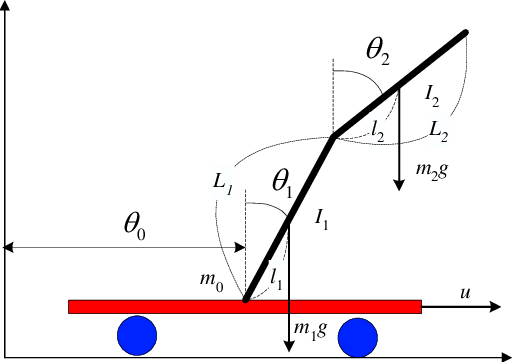
\includegraphics[width=0.4\textwidth]{figures/Double-inverted-pendulum-on-a-cart.png} % Replace "example-image" with the actual image file name and path
  \caption{Double inverted pendulum on a cart\cite{bogdanov2004optimal}}
  \label{fig:DIPC}
\end{figure}

Another significant variation is the Furuta pendulum\cite{cazzolato2011dynamics}, initially developed at the Tokyo Institute of Technology by Furuta and his colleagues\cite{furuta1992swing}. This system comprises a driven arm that rotates horizontally and a pendulum attached to this arm, allowing free vertical rotation. Due to the influence of gravitational forces and the coupling stemming from Coriolis and centripetal forces, the Furuta pendulum is characterized by its underactuation and highly nonlinear behavior.

\begin{figure}[H]
  \centering
  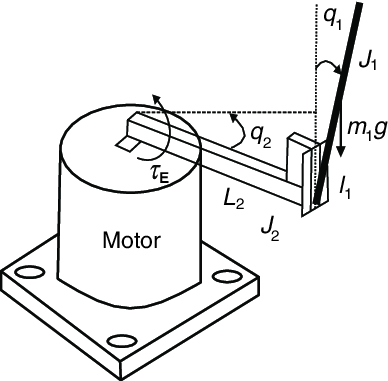
\includegraphics[width=0.4\textwidth]{figures/Furuta-pendulum.png} % Replace "example-image" with the actual image file name and path
  \caption{Furuta pendulum\cite{aguilar2010direct}}
  \label{fig:Furuta pendulum}
\end{figure}

The double pendulum utilized in this thesis represents a third variation. It consists of two links connected in series by revolute joints. Unlike the Furuta pendulum, both links of the double pendulum move in the same plane within three-dimensional space. These two links are connected to the world frame via revolute joints as well. In contrast to the DIPC setup, the actuation capability is solely limited by the torque that the joints can generate, unrestricted by the length of a prismatic rail. The dynamics of the double pendulum system will be discussed in the following section.

\subsection{Dynamics of underactuated double pendulum system}
As shown in Figure \ref{fig:double pendulum dynamics}, we model the dynamics of the double pendulum with 15 parameters which include 8 link parameters namely masses \((m_1,m_2)\)
, lengths \((l_1,l_2)\)
, center of masses \((r_1,r_2)\) 
, inertias \((I_1,I_2)\)
 for the two links, and 6 actuator parameters namely motor inertia \(I_r\)
, gear ratio \(g_r\)
, coulomb friction \((c_{f1},c_{f2})\)
, viscous friction \((b_1,b_2)\)
 for the two joints and gravity.
\begin{figure}[h]
  \centering
  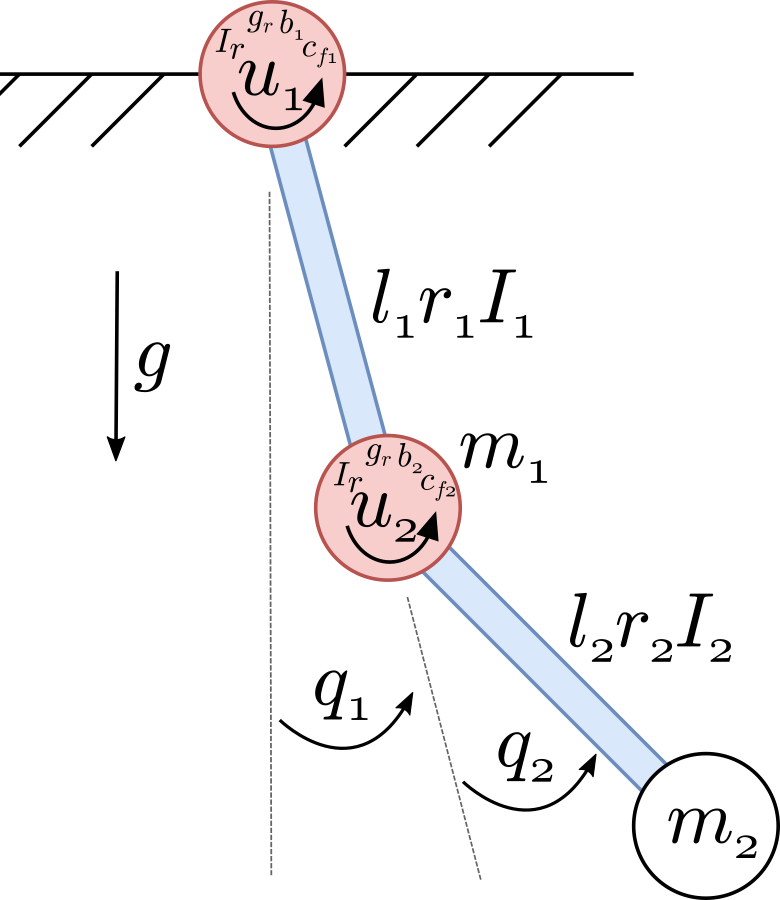
\includegraphics[width=0.5\textwidth]{figures/double_pendulum_dynamics.png} % Replace "example-image" with the actual image file name and path
  \caption{Double pendulum dynamics}
  \label{fig:double pendulum dynamics}
\end{figure}

The generalized coordinates \( \mathbf{q} =[q_1,q_2]^T \) are the joint angles measured from the free hanging position. The state vector of the systems contains the position coordinates and their time derivatives: \(\mathbf{x}=[\mathbf{q},\mathbf{\dot{q}}]^T\). The torque applied by the actuators are \(\mathbf{u}=[u_1,u_2]\). The equation of motion for the dynamics of a dynamical system can be derived following the blow steps:

\textbf{Step 1. Define the Lagrangian (\(L\)):}

   The Lagrangian (\(L\)) is defined as the difference between the kinetic energy (\(T\)) and the potential energy (\(U\)) of the system:
   \begin{align}
         L = T - U
   \end{align}


\textbf{Step 2. Express the Kinetic Energy (\(T\)):}

   The kinetic energy (\(T\)) of the double pendulum is the sum of the kinetic energies of both links. The kinetic energy for a link is given by:
   \begin{align}
        \label{eq:kinetic energy}
        T = \frac{1}{2} m_1 (\dot{x}_1^2 + \dot{y}_1^2) + \frac{1}{2} m_2 (\dot{x}_2^2 + \dot{y}_2^2)
   \end{align}

   where \(m_1\) and \(m_2\) are the masses of the links, \((x_1, y_1)\) and \((x_2, y_2)\) are their positions, and \(\dot{x}_1, \dot{y}_1, \dot{x}_2, \dot{y}_2\) are their respective velocities.

\textbf{Step 3. Express the Potential Energy (\(U\)):}

   The potential energy (\(U\)) of the double pendulum is the sum of the potential energies of both links. The potential energy for a link in a gravitational field is given by:
   \begin{align}
         \label{eq:potential energy}
         U = m_1 g y_1 + m_2 g y_2
   \end{align}

   where \(g\) is the acceleration due to gravity.
   
   
\textbf{Step 4. Formulate the Lagrange's Equation:}

   Use Lagrange's equation to derive the equations of motion for the generalized coordinates \(x_1, y_1, x_2, y_2\).

    \begin{align}
    \label{eq:lagrange equation}
    \frac{d}{dt} \left(\frac{\partial L}{\partial \dot{q_i}}\right) - \frac{\partial L}{\partial q_i} = 0
    \end{align}

\textbf{Step 5. Solve the Equations of Motion:}

   Solve the obtained set of second-order differential equations to determine the equations of motion for the system. The system dynamics with friction is:
   
   \begin{align}
        \label{eq:EoM}
        M(q)\ddot{q} + C(q,\dot{q})\dot{q} &= Du + G(q) - F(\dot{q})
   \end{align}
    
    Because the state vector is \(\mathbf{x}=[\mathbf{q},\mathbf{\dot{q}}]^T\), the equation of motion can also be expressed as:
    
    \begin{equation}
    \begin{split}
        \dot{x} &= f(x,u) \\
        &= \begin{bmatrix} 
            \dot{q} \\ 
            M^{-1}(Du - C(q,\dot{q})\dot{q} + G(q) - F(\dot{q})) 
       \end{bmatrix}
    \end{split}
    \end{equation}

   Consider the forward kinematics of double pendulum system, the coordinate of the joint between the first link and the second link is \(P_1=(x_1,y_1)\),the coordinate of the end effector is \(P_2=(x_2,y_2)\).

    \begin{align}
        \label{eq:p1}
        \left\{
        \begin{aligned}
        x_1 &= l_1 \sin(q_1) \\
        y_1 &= - l_1 \cos(q_1)
        \end{aligned}
        \right.
    \end{align}

    \begin{align}
        \label{eq:p2}
        \left\{
        \begin{aligned}
        x_2 &= l_1 \sin(q_1) + l_2 \sin(q_1 + q_2) \\
        y_2 &= -l_1 \cos(q_1) - l_2 \cos(q_1 + q_2)
        \end{aligned}
        \right.
    \end{align}

    Put Equation \ref{eq:p1} and \ref{eq:p2} into \ref{eq:kinetic energy}, \ref{eq:potential energy}, \ref{eq:lagrange equation}, \ref{eq:EoM},we can get the mass matrix (with \(s_1 = \sin(q_1), c_1 = \cos(q_1), \ldots\))
    \begin{equation}
    \mathbf{M} =
    \left[ 
    {\begin{array}{cc}
    I_1 + I_2 + l_1^2m_2 + 2l_1m_2r_2c_2 + g_r^2I_r + I_r  &   I_2 + l_1m_2r_2c_2 - g_rI_r  \\
    I_2 + l_1m_2r_2c_2 - g_rI_r                    & I_2 + g_r^2I_r                       \\
    \end{array}} 
    \right]
    \end{equation}
    
    The Coriolis matrix:
    
    \begin{equation}
    \begin{split}
    \mathbf{C} = \left[
    \begin{matrix}
    -2 \dot{q}_2 l_{1} m_{2} r_{2} \sin(q_2) & -\dot{q}_2 l_{1} m_{2} r_{2} \sin(q_2)\\
    \dot{q}_1 l_{1} m_{2} r_{2} \sin(q_2) & 0
    \end{matrix}
    \right],
    \label{eq:coriolis_matrix}
    \end{split}
    \end{equation}
    
    The gravity vector:
    
    \begin{equation}
    \begin{split}
    \mathbf{G} = \left[
    \begin{matrix}
    - g m_{1} r_{1} \sin(q_1) - g m_{2} \left(l_{1} \sin(q_1) + r_{2} \sin(q_{1+2}) \right) \\
    - g m_{2} r_{2} \sin(q_{1+2})
    \end{matrix}
    \right],
    \label{eq:gravity_matrix}
    \end{split}
    \end{equation}
    
    The friction vector:
    
    \begin{equation}
        \begin{split}
            \mathbf{F} =
            \left[
                \begin{matrix}
                    b_1 \dot{q}_1 + c_{f1} \arctan(100\,\dot{q}_1) \\
                    b_2 \dot{q}_2 + c_{f2} \arctan(100\,\dot{q}_2)
                \end{matrix}
            \right]
        \end{split}
    \end{equation}
    (the \(\arctan(100\,\dot{q}_i)\) function is used to approximate the discrete step function for the coulomb friction)

    And the actuator selection matrix \(\mathbf{D}\):
    
    \begin{equation}
        \begin{split}
            \mathbf{D}_{full} =
            \left[
                \begin{matrix}
                    1 & 0 \\
                    0 & 1
                \end{matrix}
            \right],
            \quad
            \mathbf{D}_{pendu} =
            \left[
                \begin{matrix}
                    1 & 0 \\
                    0 & 0
                \end{matrix}
            \right],
            \quad
            \mathbf{D}_{acro} =
            \left[
                \begin{matrix}
                    0 & 0 \\
                    0 & 1
                \end{matrix}
            \right]
        \end{split}
    \end{equation}
    
    for the fully actuated system, the pendubot or the acrobot.

\section{Related work}
This thesis focuses on learning-based robotic motion control, a field that has garnered increasing attention in recent years, with significant contributions from various research institutes.

Today, much of the research in this field is conducted within simulation environments due to their cost-effectiveness and the ability to facilitate rapid iteration. One noteworthy project from 2018 is the DeepMimic project\cite{peng2018deepmimic}, undertaken by researchers at the University of California, Berkeley. This work resides at the intersection of deep reinforcement learning, imitation learning, and robotics.

The DeepMimic project utilizes physics-based simulations to successfully replicate the diverse range of behaviors exhibited in the real world by 3D characters. These characters include real-world examples such as humanoid and Atlas robotics, as well as fictional characters like T-Rexes and dragons. Instead of relying on manually designed controllers, the project employs deep reinforcement learning methods to generalize to new skills and situations, often without human intervention.

In the training process, the agent being trained is provided with reference data recorded by motion capture actors or keyframed animations. Through imitation learning, the agent is guided to achieve specific predefined goals. The central contribution of this project lies in its framework, which combines goal-directed reinforcement learning with reference data generated by humans. This combination enables the imitation of a wide variety of motion skills.

\begin{figure}[H]
  \centering
  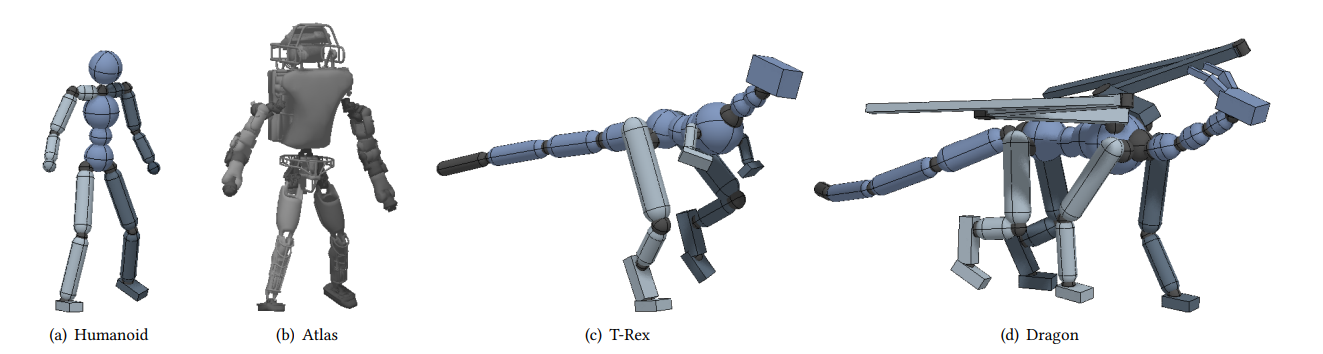
\includegraphics[width=1.0\textwidth]{figures/deepmimic.png} % Replace "example-image" with the actual image file name and path
  \caption{3D characters in Deepmimic project\cite{peng2018deepmimic}}
  \label{fig:deepmimic}
\end{figure}

In the context of reinforcement learning, a distinction exists between model-free and model-based approaches. Model-free reinforcement learning does not require information about the transition model, whereas model-based reinforcement learning leverages the transition model to make decisions based on a prior known model or one learned from interactions.

The model-free approach is notably characterized by its sample inefficiency. Successful training often takes many hours, if not days or weeks.

An intriguing project that relies solely on model-free deep reinforcement learning is the Learning-to-Walk-in-20 Minutes project\cite{smith2022walk} conducted by researchers from UC Berkeley. They employ an algorithmic framework closely related to DroQ \cite{hiraoka2021dropout}, an extension of the SAC algorithm \cite{haarnoja2018soft} incorporating dropout \cite{srivastava2014dropout} and layer normalization \cite{ba2016layer}. Remarkably, their training is conducted directly on the real system. They demonstrate that current deep RL methods can effectively teach quadrupedal locomotion in under 20 minutes, a stark contrast to previous research conducted by Kumar et al. \cite{kumar2021rma}, which employed the same hardware but required \(1.2 \times 10^9\) samples to train a robust controller for locomotion. This corresponds to roughly 4.5 months' worth of cumulative experience.


Additionally, a research team from ETH Zurich has made significant progress in addressing the sim-to-real interface challenge \cite{hwangbo2019learning}. Their methodology involves training a control model for a mini-cheetah-like robot within a simulation environment. By utilizing a neural network and leveraging data collected from the real robot, they approximated the dynamics model of the physical robot. This approach has facilitated accurate implementation of the control policy derived from the virtual environment onto the real robot. These exemplary works demonstrate the promising applications of learning-based approaches in various aspects of robot control.

\cleardoublepage
